\section{Công trình liên quan}

\begin{frame}{Các phương pháp cho bài toán sinh cử chỉ}

%\textbf{Rule Base \& Statistic}
%\begin{itemize}
%	\item BEAT, Rule-based generation  \cite{cassell2001beat}
%	\item Gesture Controllers  \cite{levine2010gesture}
%\end{itemize}
%%	\textit{Nhược điểm}: Không có khả năng mở rộng, kết quả không tốt với các dữ liệu ngoài tập huấn luyện.
%
%\textbf{Deep Learning}
%\begin{columns}
%	\begin{column}{0.5\textwidth}
%			{
%			\textbf{Likelihood-based models}:
%			\begin{itemize}
%				\item \textbf{MLP}: Gesticulator,  \textbf{RNN}: Speech2AffectiveGestures, HA2G, TransGesture, .. 
%				\item \textbf{Normalising Flows}: Text2gestures, Speech2Gesture
%				\textbf{VAE/VQ-VAE}:  Audio2Gestures; 
%				\end{itemize}
%			}
%			 \begin{figure}
%				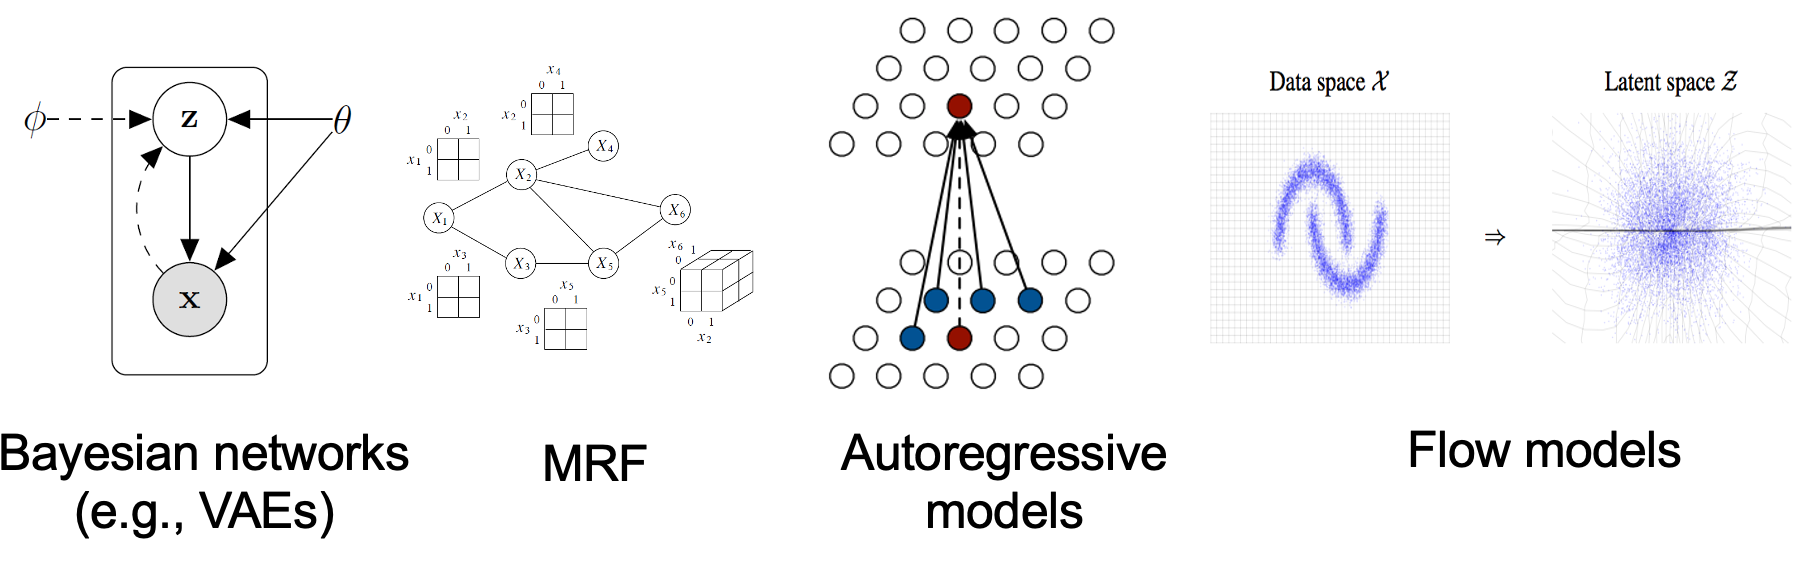
\includegraphics[width=\textwidth]{likelihood_based_models}
%			\end{figure}
%	\end{column}
%	\hspace{-20pt}
%	\begin{column}{0.5\textwidth}
%		{
%			\textbf{Implicit generative models}:
%\begin{itemize}
%			\item \textbf{GAN}: DiffGAN
%			
%			\item \textbf{Diffusion}: Listen denoise action \cite{alexanderson2023listen}, \textit{DiffuseStyleGesture} \cite{yang2023diffusestylegesture}, Taming Diffusion \cite{zhu2023taming}.
% \end{itemize}
% 
% \begin{figure}
% 	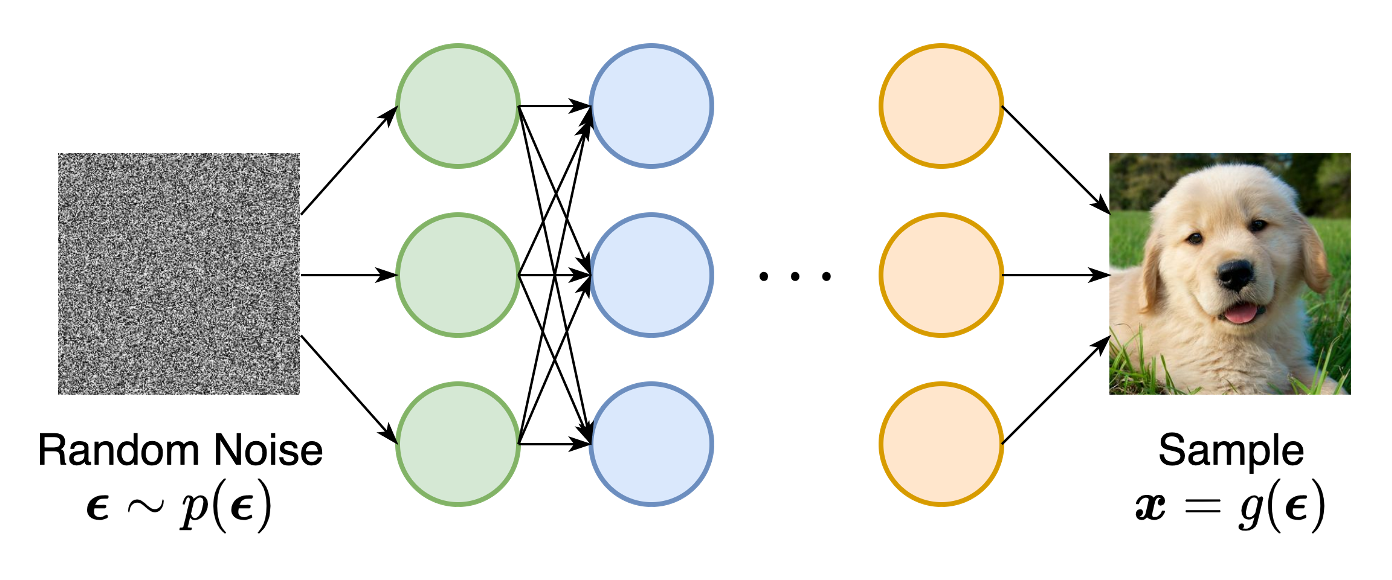
\includegraphics[width=\textwidth]{implicit_models}
% \end{figure}
% 
%		}
%	\end{column}
%\end{columns}
\begin{figure}[width=\textwidth]
	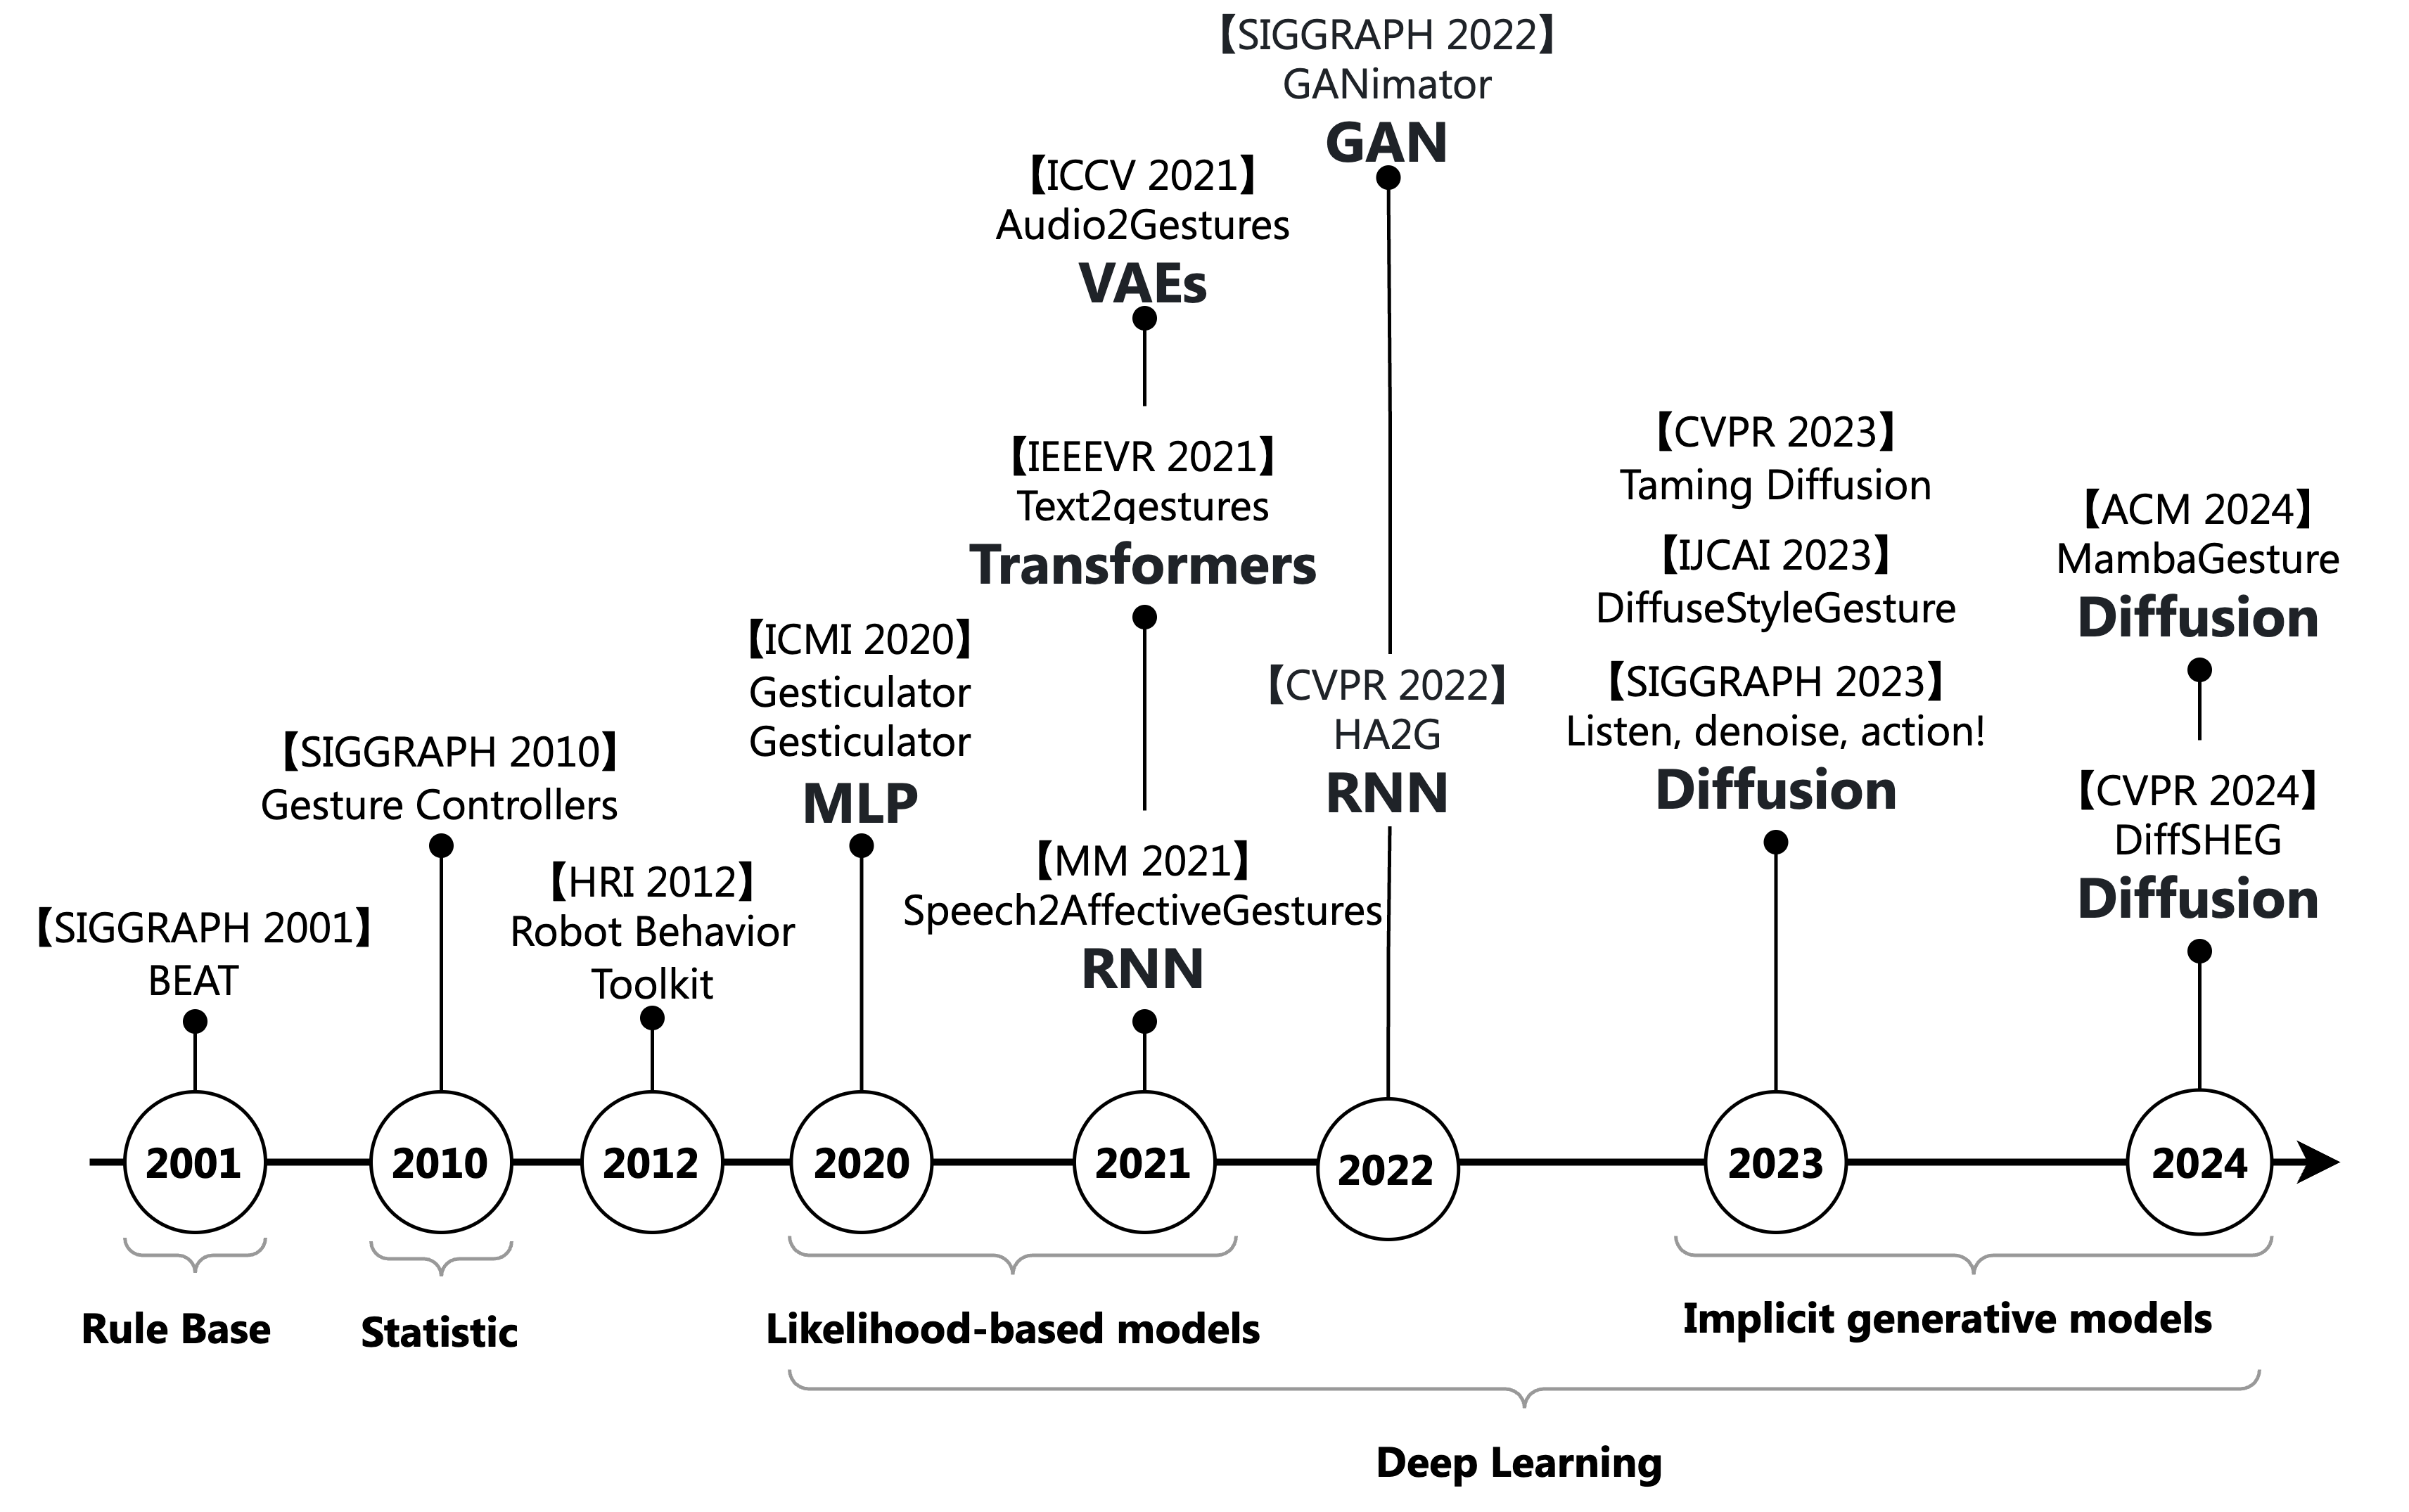
\includegraphics[width=\textwidth]{Timeline}
\end{figure}
\end{frame}


\begin{frame}{Bảng so sánh các phương pháp}
	
%	\begin{table}[h!]
%		\small
%		\centering
%		\renewcommand{\arraystretch}{1.5} % Tăng khoảng cách giữa các hàng
%		\begin{tabular}{|p{0.2\textwidth}|p{0.15\textwidth}|p{0.55\textwidth}|}
%			\hline
%			\textbf{Phương pháp} & \textbf{Loại} & \textbf{Mô tả} \\ \hline
%			BEAT & Learning-Based & Phương pháp tạo chuyển động bậc thang sử dụng các mô hình huấn luyện như CNN, RNN, và Transformer, kết hợp nhiều mô thức như âm thanh, văn bản, và biểu cảm khuôn mặt. \\ \hline
%			DisCO & Learning-Based & Tách biệt chuyển động thành các đặc trưng ẩn như nội dung và nhịp điệu, sử dụng giải mã chuyển động để tạo ra các cử chỉ. \\ \hline
%			EMAGE & Learning-Based & Sử dụng "Masked Gesture Reconstruction" (MG2G) và "Audio-Conditioned Gesture Generation" (A2G) để tạo ra các chuyển động khuôn mặt và cơ thể dựa trên các đặc trưng được huấn luyện trước. \\ \hline
%			TalkSHOW & Learning-Based & Phương pháp sử dụng autoencoder để tạo ra chuyển động khuôn mặt và VQ-VAE cho chuyển động cơ thể và tay, cùng mô hình autoregressive để dự đoán chuyển động tương lai. \\ \hline
%			Liu et al. (CaMN) & Learning-Based & Mạng Cascade Motion Network (CaMN) tạo ra các cử động cơ thể và tay, sử dụng huấn luyện đối kháng qua nhiều mô thức. \\ \hline
%			Yoon et al. & Learning-Based & Xử lý tạo cử chỉ như một bài toán dịch, sử dụng RNN với ngữ cảnh đa phương thức của âm thanh, văn bản, và danh tính người nói. \\ \hline
%		\end{tabular}
%	\end{table}

\begin{table}[h!]
	\footnotesize
	\centering
	\renewcommand{\arraystretch}{1.5} % Tăng khoảng cách giữa các hàng
	\begin{tabular}{|p{0.2\textwidth}|p{0.15\textwidth}|p{0.55\textwidth}|}
		\hline
		\textbf{Phương pháp tiêu biểu} & \textbf{Loại} & \textbf{Nguyên lý} \\ \hline
		Robot behavior toolkit & Rule-Based & Tạo một tập hợp các đơn vị cử chỉ và thiết kế các Rule cụ thể để ánh xạ lời nói thành một chuỗi các đơn vị cử chỉ. \\ \hline
		Gesture Controller & Statistical Models & Sử dụng mô hình xác suất như Hidden Markov Models (HMM) để mô hình hóa phân phối cử chỉ bằng cách phân tích các thống kê. \\ \hline
		Gesticulator(\textbf{MLP}), HA2G (\textbf{RNN}), Text2Gestures (\textbf{Transformers}) & Likelihood-Based & Sử dụng neural network  (MLP, RNN, Transformers) để học end-to-end quan hệ của cử chỉ và âm thanh. Coi việc sinh cử chỉ như là một quá trình tái tạo (reconstruction) dữ liệu cử chỉ ban đầu. \\ \hline
		\textbf{Diffusion}: MDM, Listen, Denoise, Action
		DiffuseStyleGesture & Implicit Generative & Học cách chuyển từ phân phối chuẩn về phân phối của dữ liệu để ngầm định việc học phân phối của dữ liệu, tạo ra sự đa dạng trong việc sinh cử chỉ. \\ \hline
	\end{tabular}
\end{table}


\end{frame}

\begin{frame}{Đánh giá các phương pháp}
	
	\begin{table}[h!]
		\footnotesize
		\centering
		\renewcommand{\arraystretch}{1.5} % Tăng khoảng cách giữa các hàng
		\begin{tabular}{|p{0.2\textwidth}|p{0.35\textwidth}|p{0.35\textwidth}|}
			\hline
			\textbf{Loại phương pháp} & \textbf{Ưu điểm} & \textbf{Nhược điểm} \\ \hline
			Rule-Based \& Statistical & 
			- Dễ hiểu và dễ triển khai. \newline 
			- Dễ giải thích và có thể kiểm soát được \newline
			- Hiệu quả trong các trường hợp đơn giản hoặc dữ liệu nhỏ. & 
			- Không tổng quát hóa tốt với dữ liệu phức tạp. \newline 
			- Đòi hỏi nhiều công sức trong việc xây dựng quy tắc thủ công. \\ \hline
%			Statistical Models & 
%			- Khả năng học mô hình từ dữ liệu. \newline 
%			- Tốt với các hệ thống tuyến tính hoặc phi tuyến tính đơn giản. & 
%			- Hiệu năng giảm với dữ liệu có độ phức tạp cao. \newline 
%			- Cần nhiều dữ liệu để huấn luyện chính xác. \\ \hline
			Likelihood-Based Models & 
			- Khả năng ước lượng mật độ xác suất của dữ liệu \newline 
			- Có khả năng mở rộng và học từ dữ liệu lớn & 
			- Dễ bị ảnh hưởng bởi nhiễu \newline 
			- Kết quả thấp ở vùng dữ liệu hiếm \newline
			- Khả năng sinh không đa dạng \\ \hline
			Implicit Generative Models & 
			- Tạo ra dữ liệu chất lượng cao. \newline 
			- Linh hoạt và đa dạng \newline
			- Phủ được vùng có mật độ dữ liệu thấp & 
			- Cần cấu hình phức tạp để đạt hiệu năng tốt. \newline 
			- Khó đánh giá do mỗi lần nhiễu là khác nhau. \newline 
			- Quá trình lấy mẫu chậm \\ \hline
		\end{tabular}
	\end{table}
	
\end{frame}

\begin{frame}{Mô hình diffusion}
	\begin{figure}
		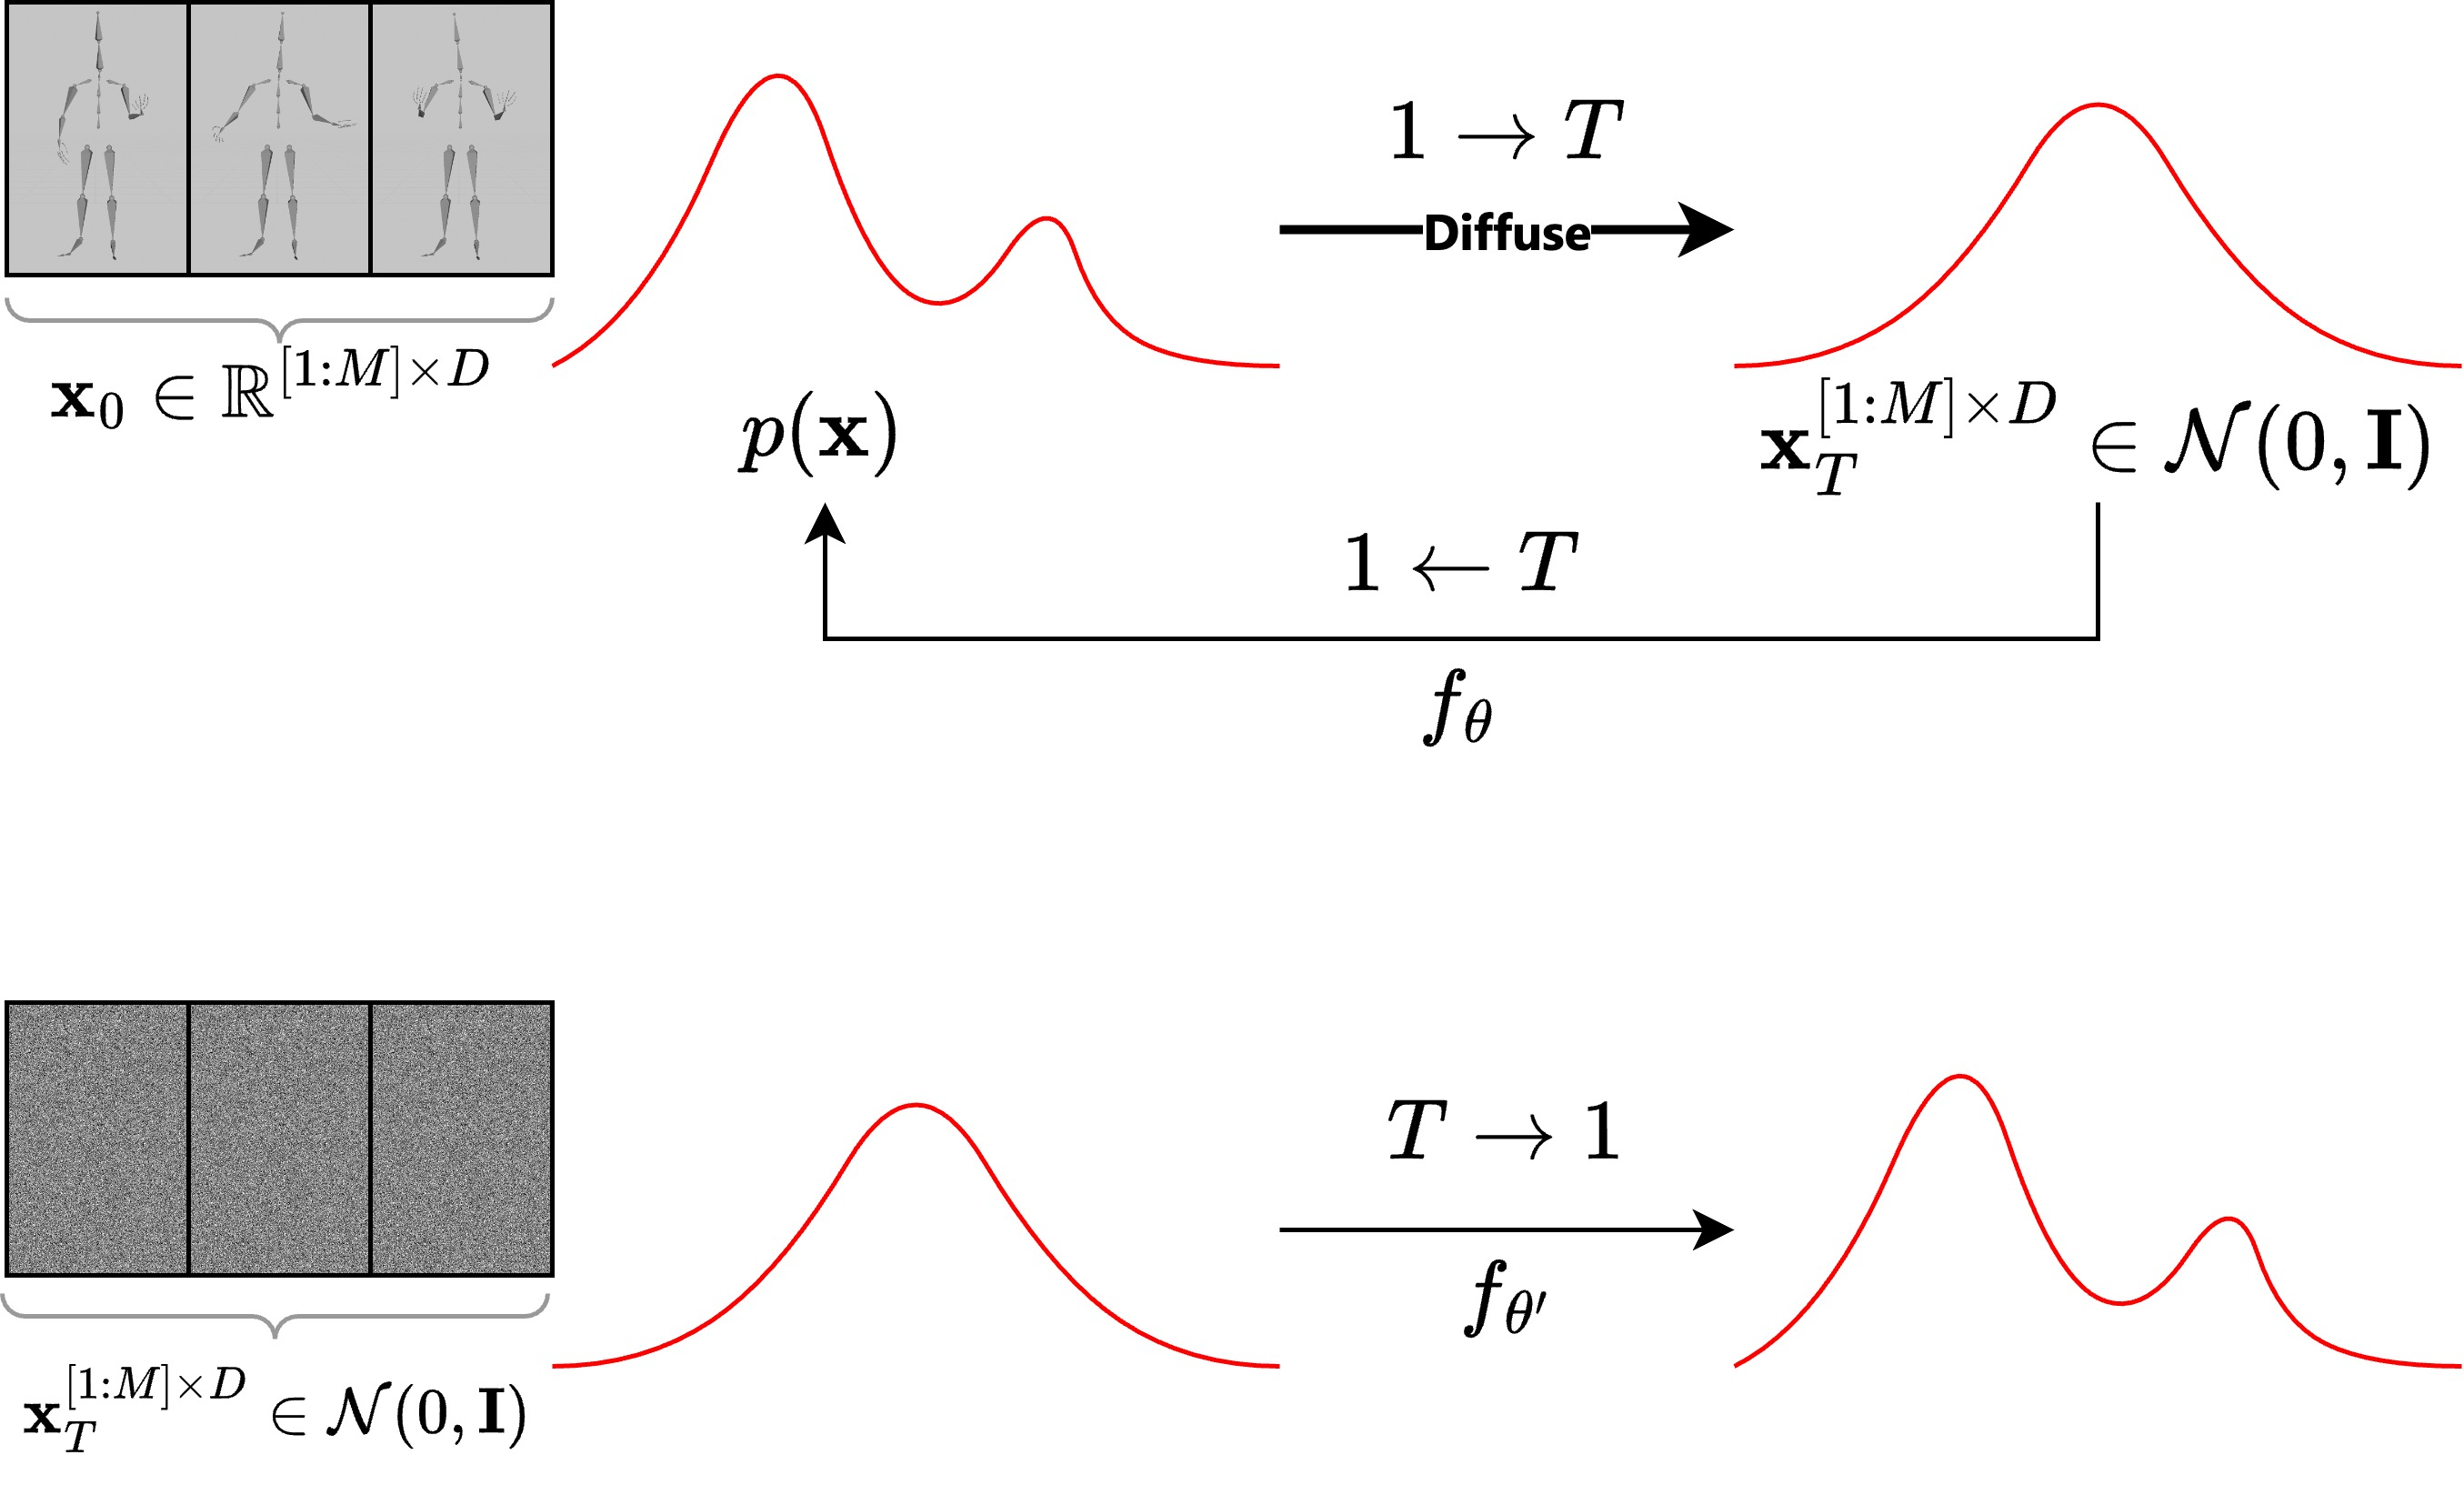
\includegraphics[width=\textwidth]{DistributionTransition}
	\end{figure}	
\end{frame}

%\begin{frame}{Tư tưởng cơ bản của Diffusion}
%	%	Dataset $\mathcal{G} = \{ x_{i}^{M \times D} \}_{1}^{n}$, ta chuẩn hóa dữ liệu $\bx_{i}^{M \times D} = \frac{\bx_{i}^{M \times D} - \mu}{\sigma}$
%	\begin{figure}
%		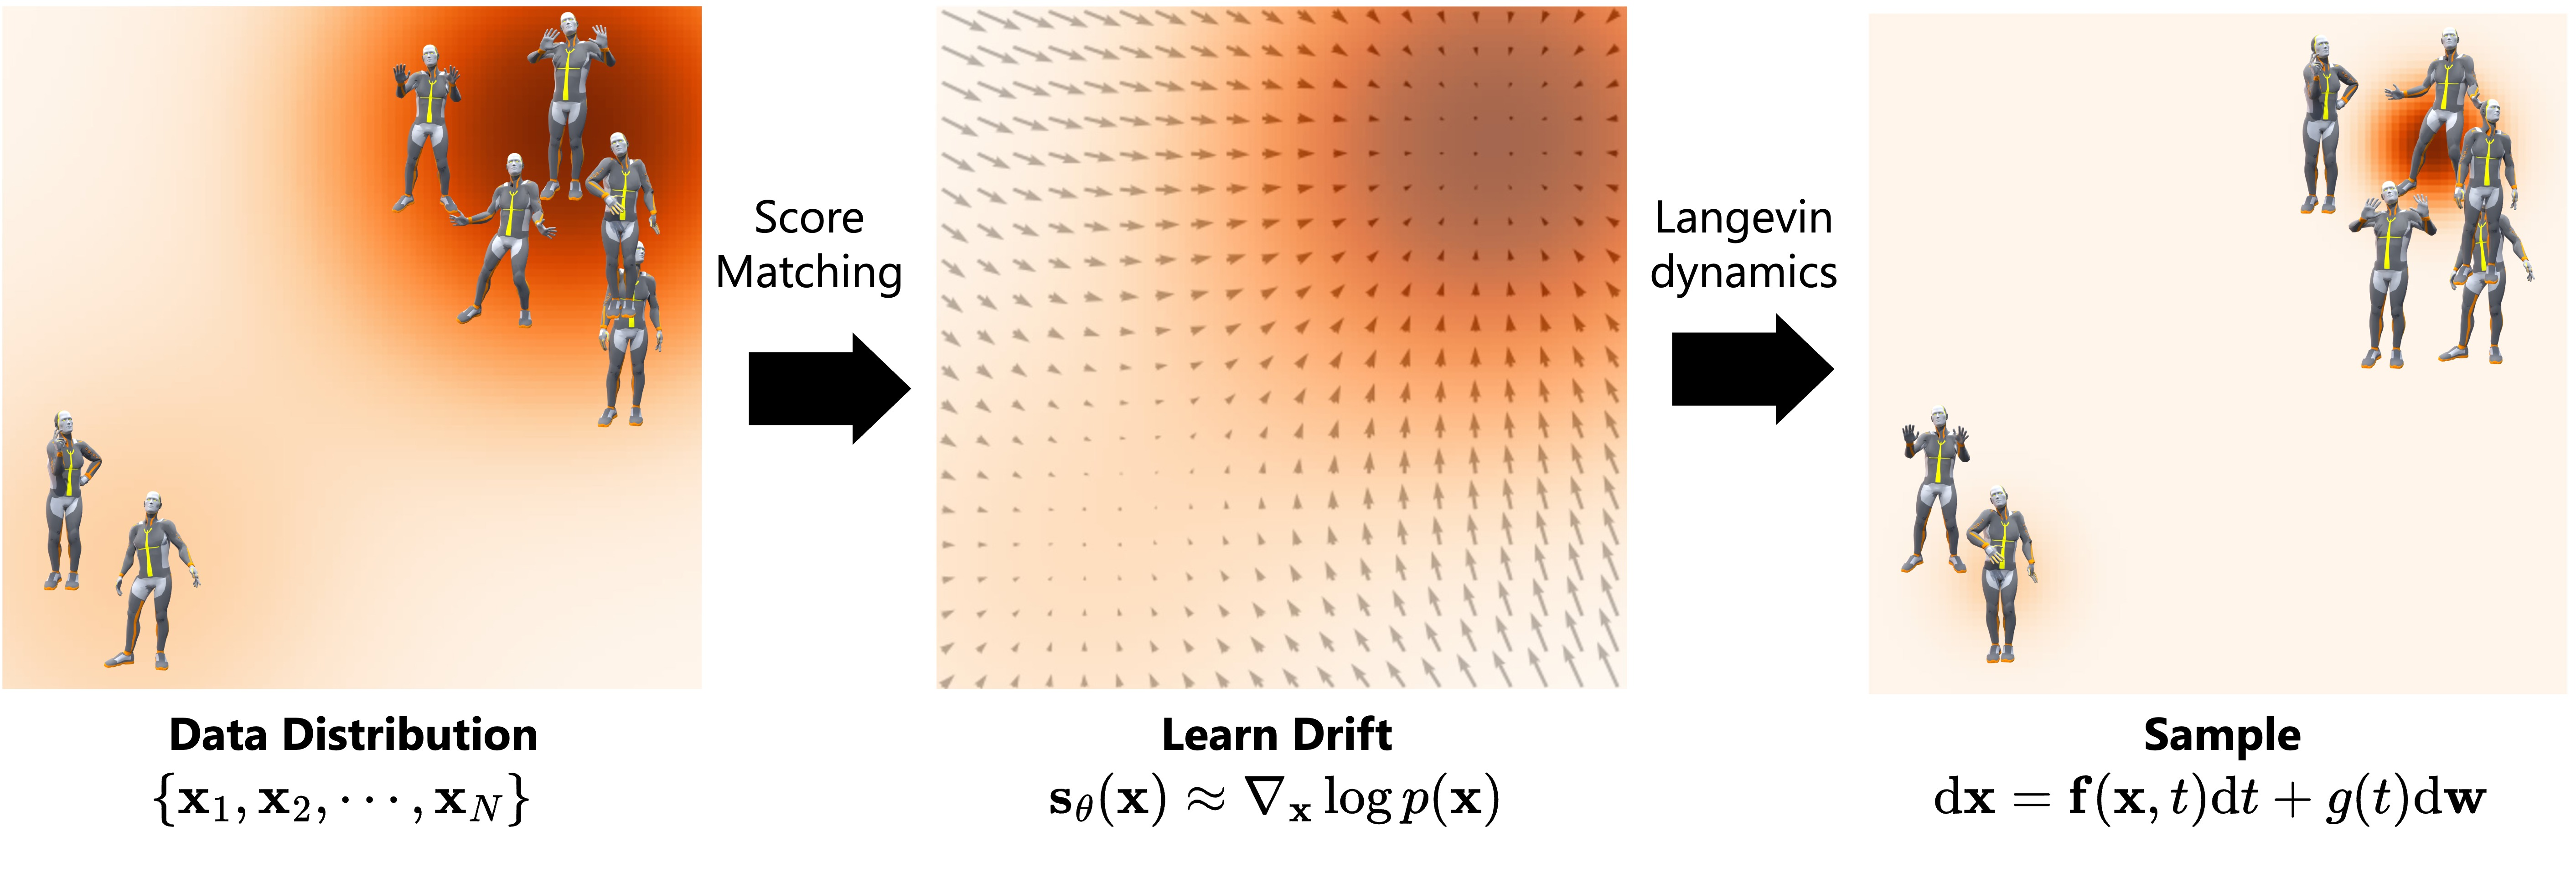
\includegraphics[width=\textwidth]{ScoreMatching}
%	\end{figure}
%\end{frame}

%\begin{frame}{Phân phối thật (Ground truth) của dữ liệu}
%\begin{figure}
%	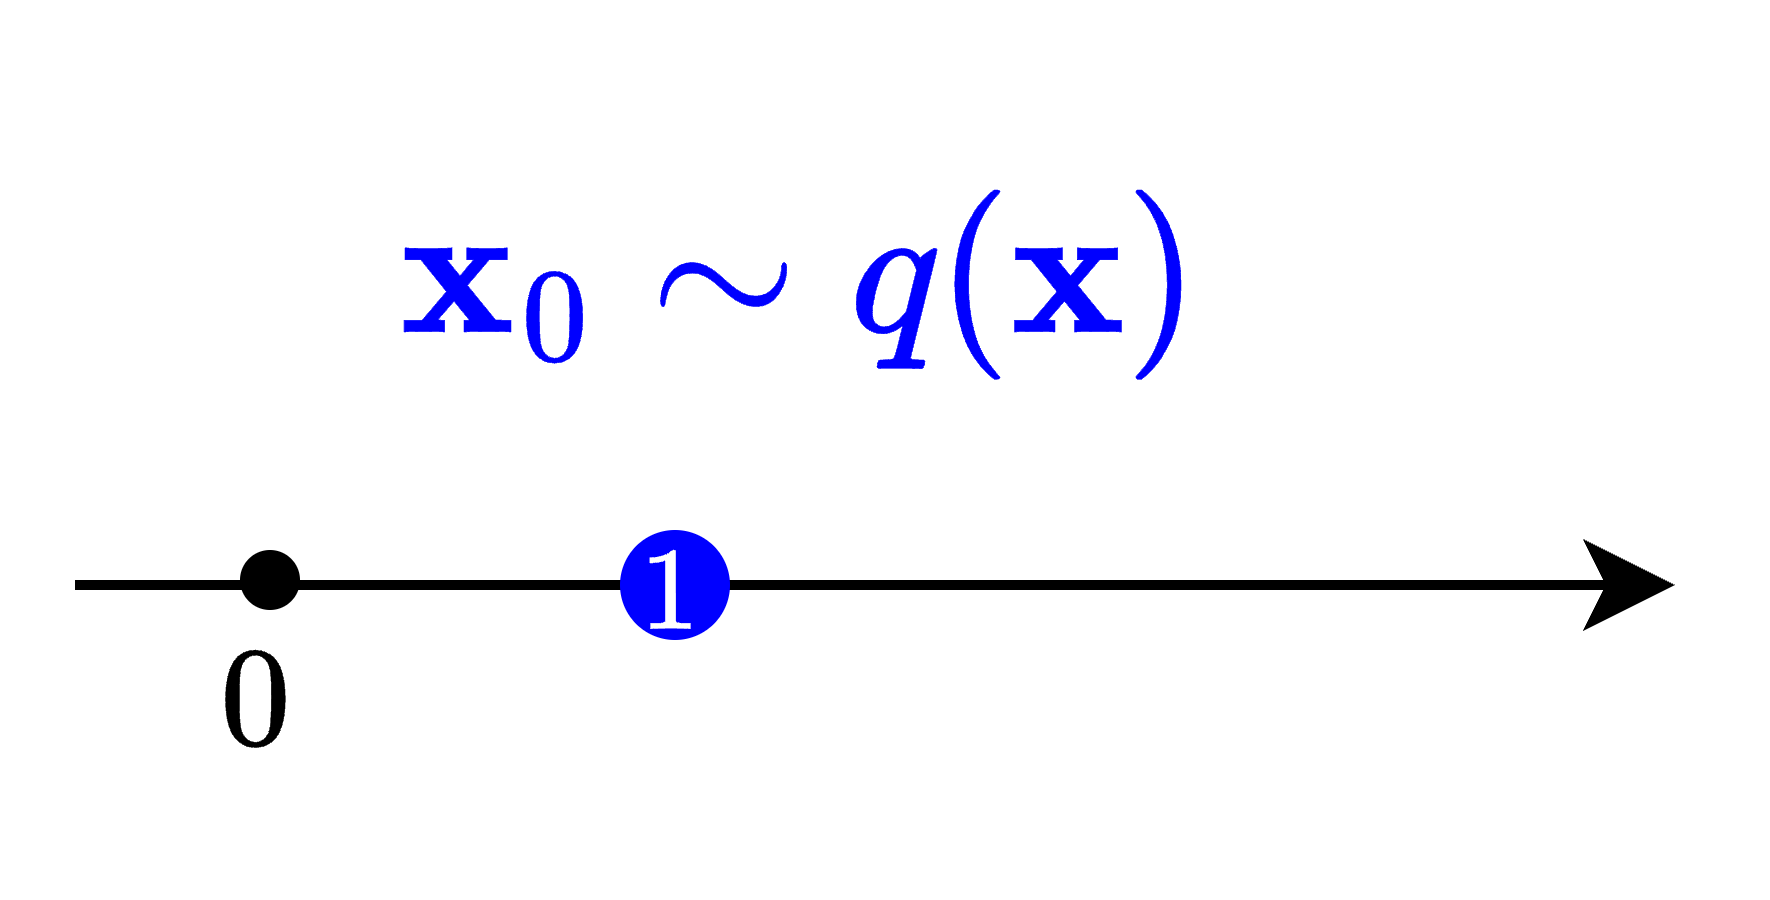
\includegraphics[width=0.9\textwidth]{ScoreDrift1}
%\end{figure}
%\end{frame}

\begin{frame}{Quá trình huấn luyện (offline)}
	\begin{figure}
		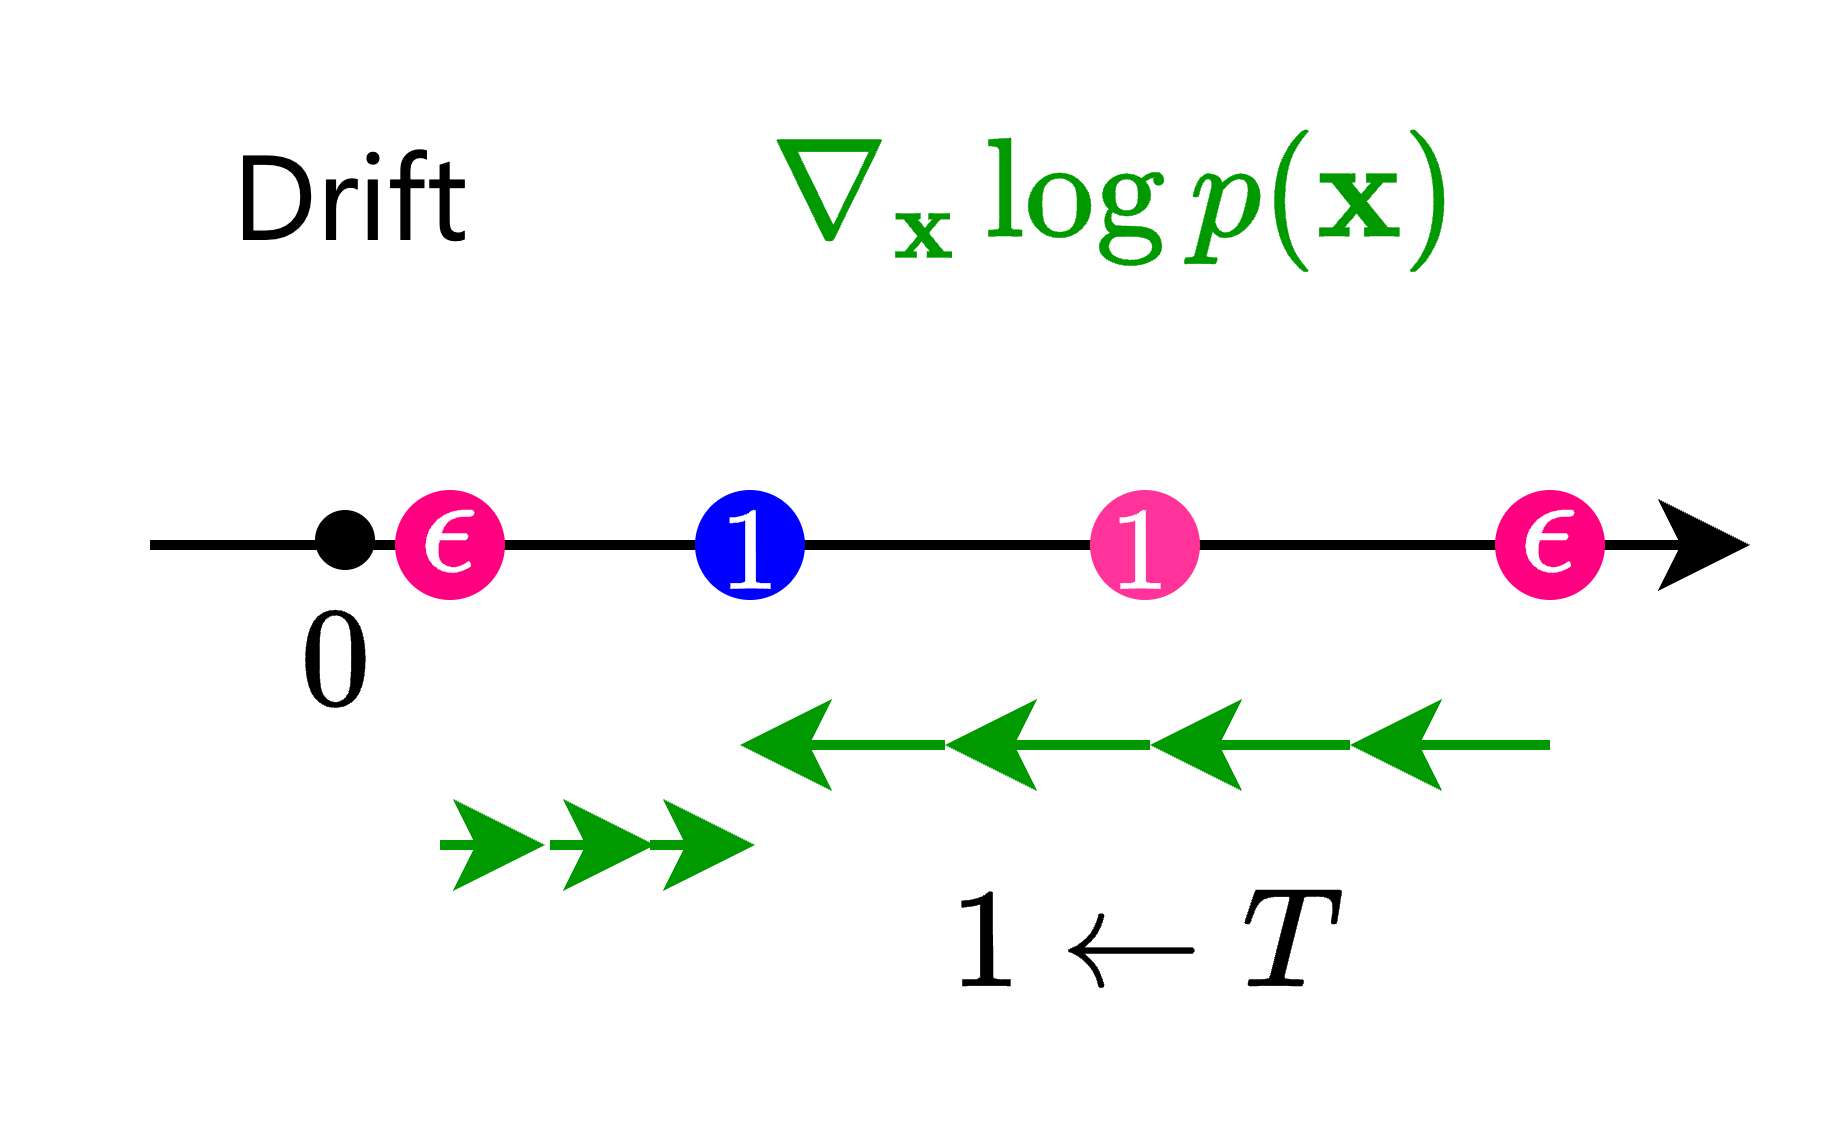
\includegraphics[width=0.9\textwidth]{ScoreDrift2}
	\end{figure}
\end{frame}
\begin{frame}{Quá trình suy luận (online)}
	\begin{figure}
		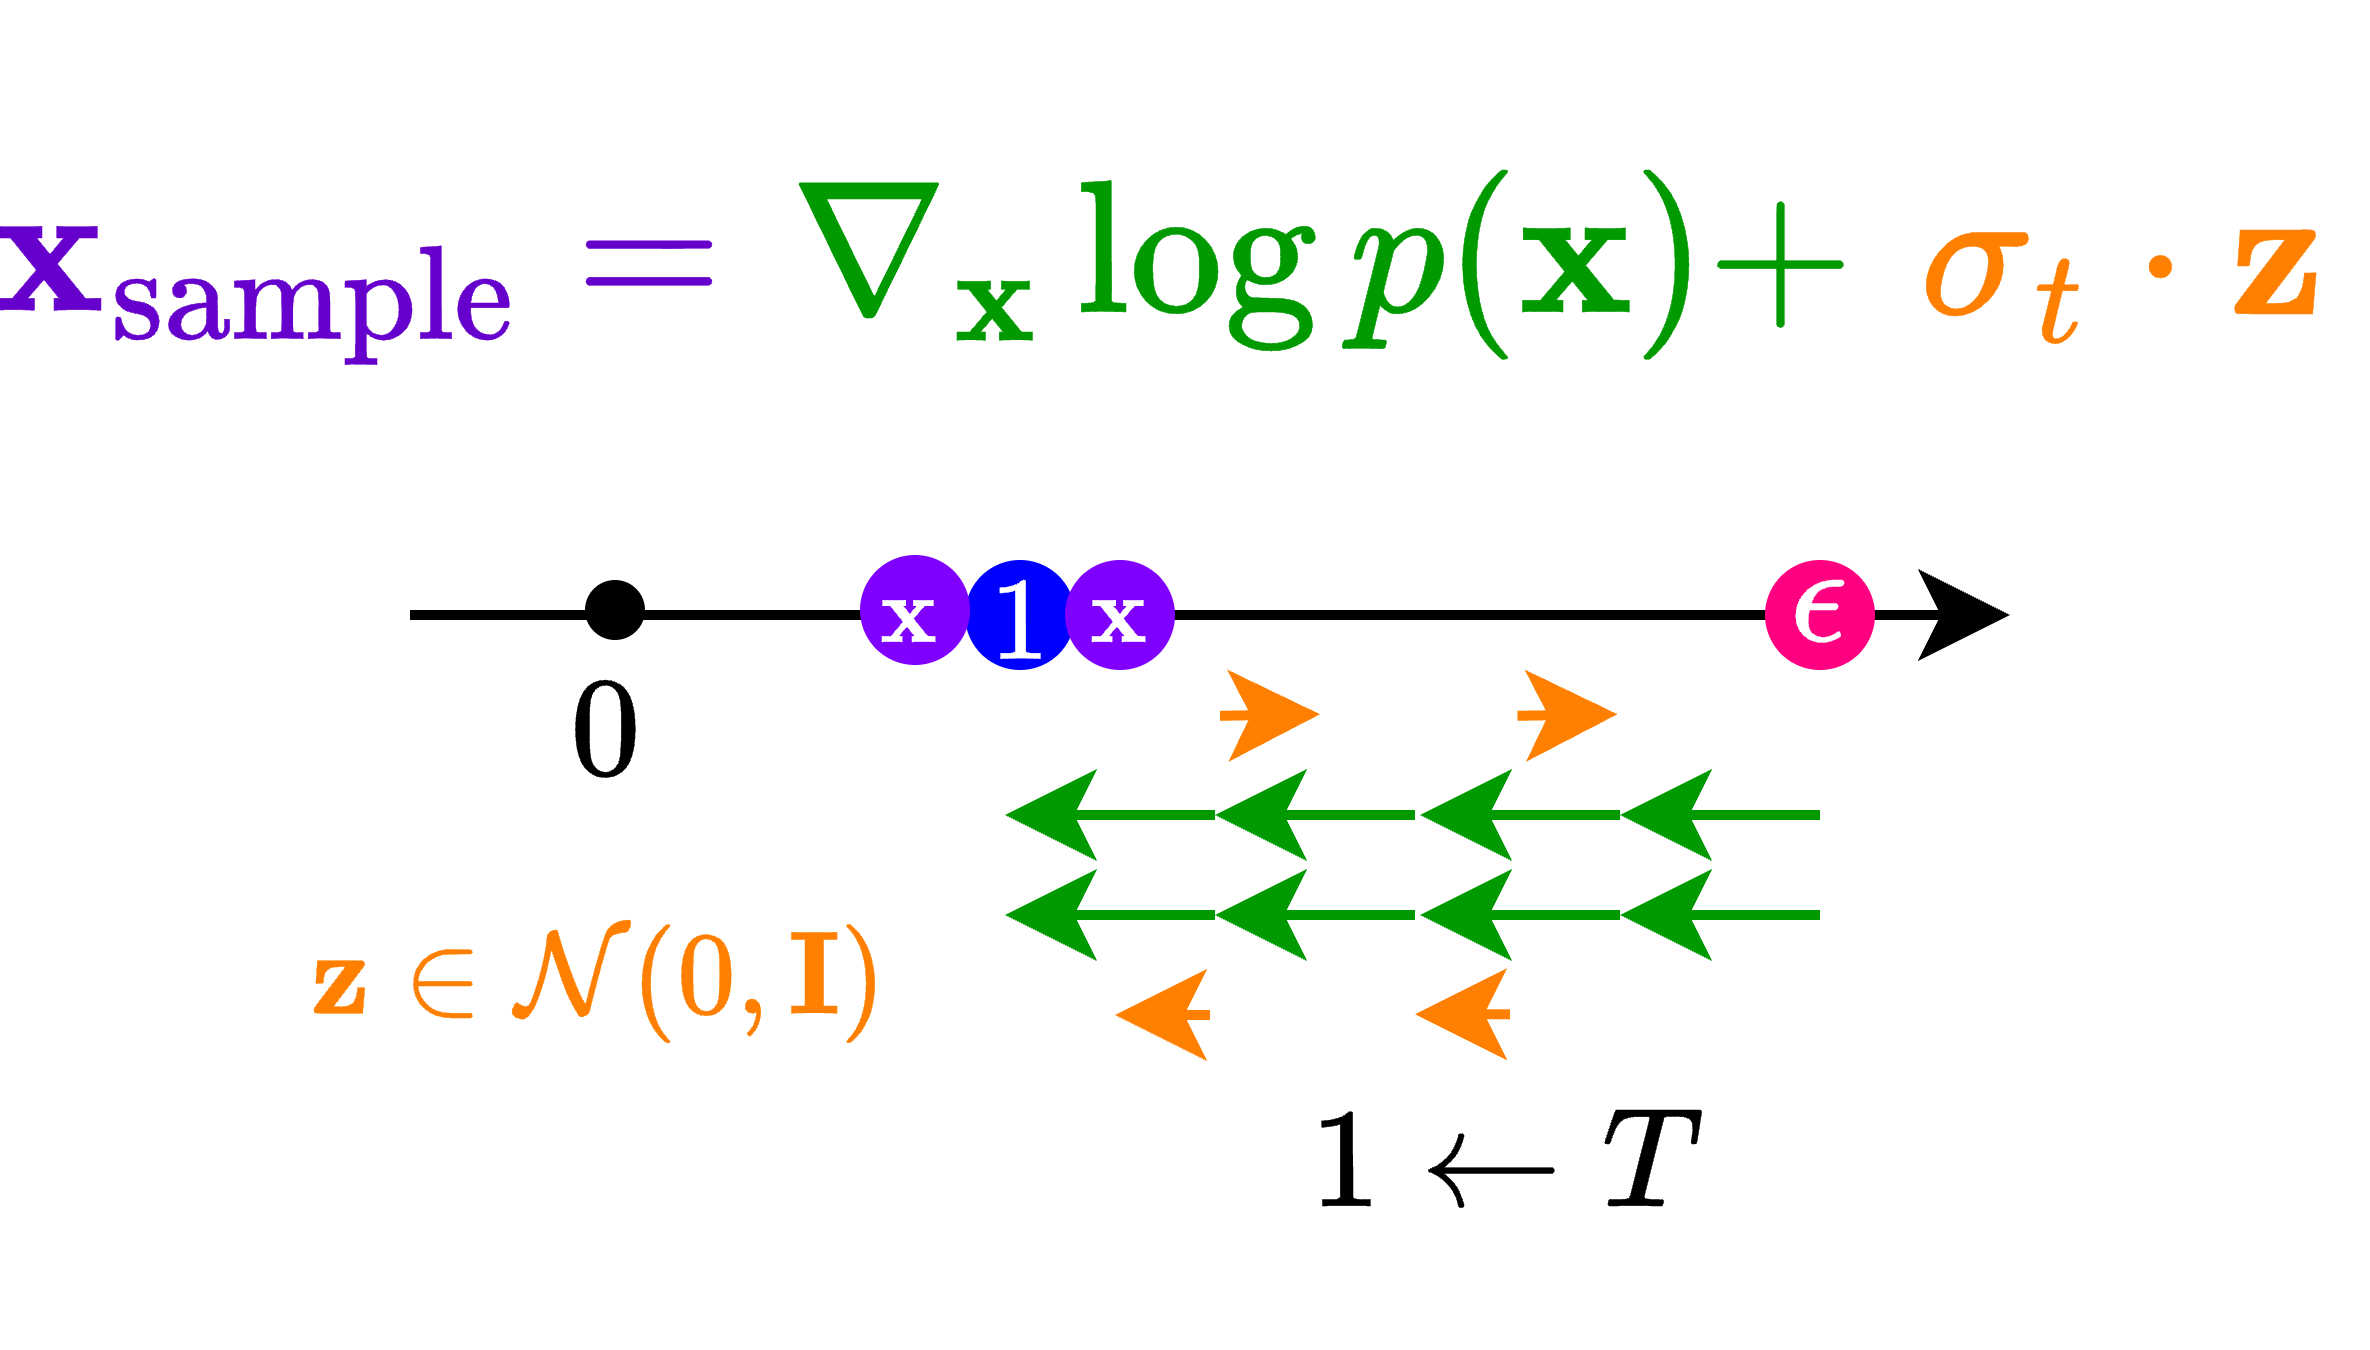
\includegraphics[width=0.9\textwidth]{ScoreDrift3}
	\end{figure}
\end{frame}


\begin{frame}{Điều khiển $\sigma_t$ bằng với Langevin dynamics}
	%	Cho $L$ là biến điều chỉnh độ lệch chuẩn
	%	 $\mathcal{N}(0, \sigma_i^2 I), i=1,2,\cdots,L$. $\mathbf{s}_\theta(\mathbf{x}, i) \approx \nabla_\mathbf{x} \log p_{\sigma_i}(\mathbf{x})$ $i= 1, 2, \cdots, L$.
	
	%	Ta dễ dàng sinh mẫu (sampling) từ ${\sigma_i}(\mathbf{x})$ bằng cách lấy mẫu $\mathbf{x} \sim p(\mathbf{x})$  và tính $\mathbf{x} + \sigma_i \mathbf{z}$ với $\mathbf{z} \sim \mathcal{N}(0, I)$

	%, hội tụ ở vùng có mật độ xác suất cao.
	
	$T \rightarrow 1$ :  $\sigma_T > \cdots  >  \sigma_2 > \sigma_1$, $\sigma_t$ sẽ giảm dần nhiễu
		
	\begin{figure}
		\centering
		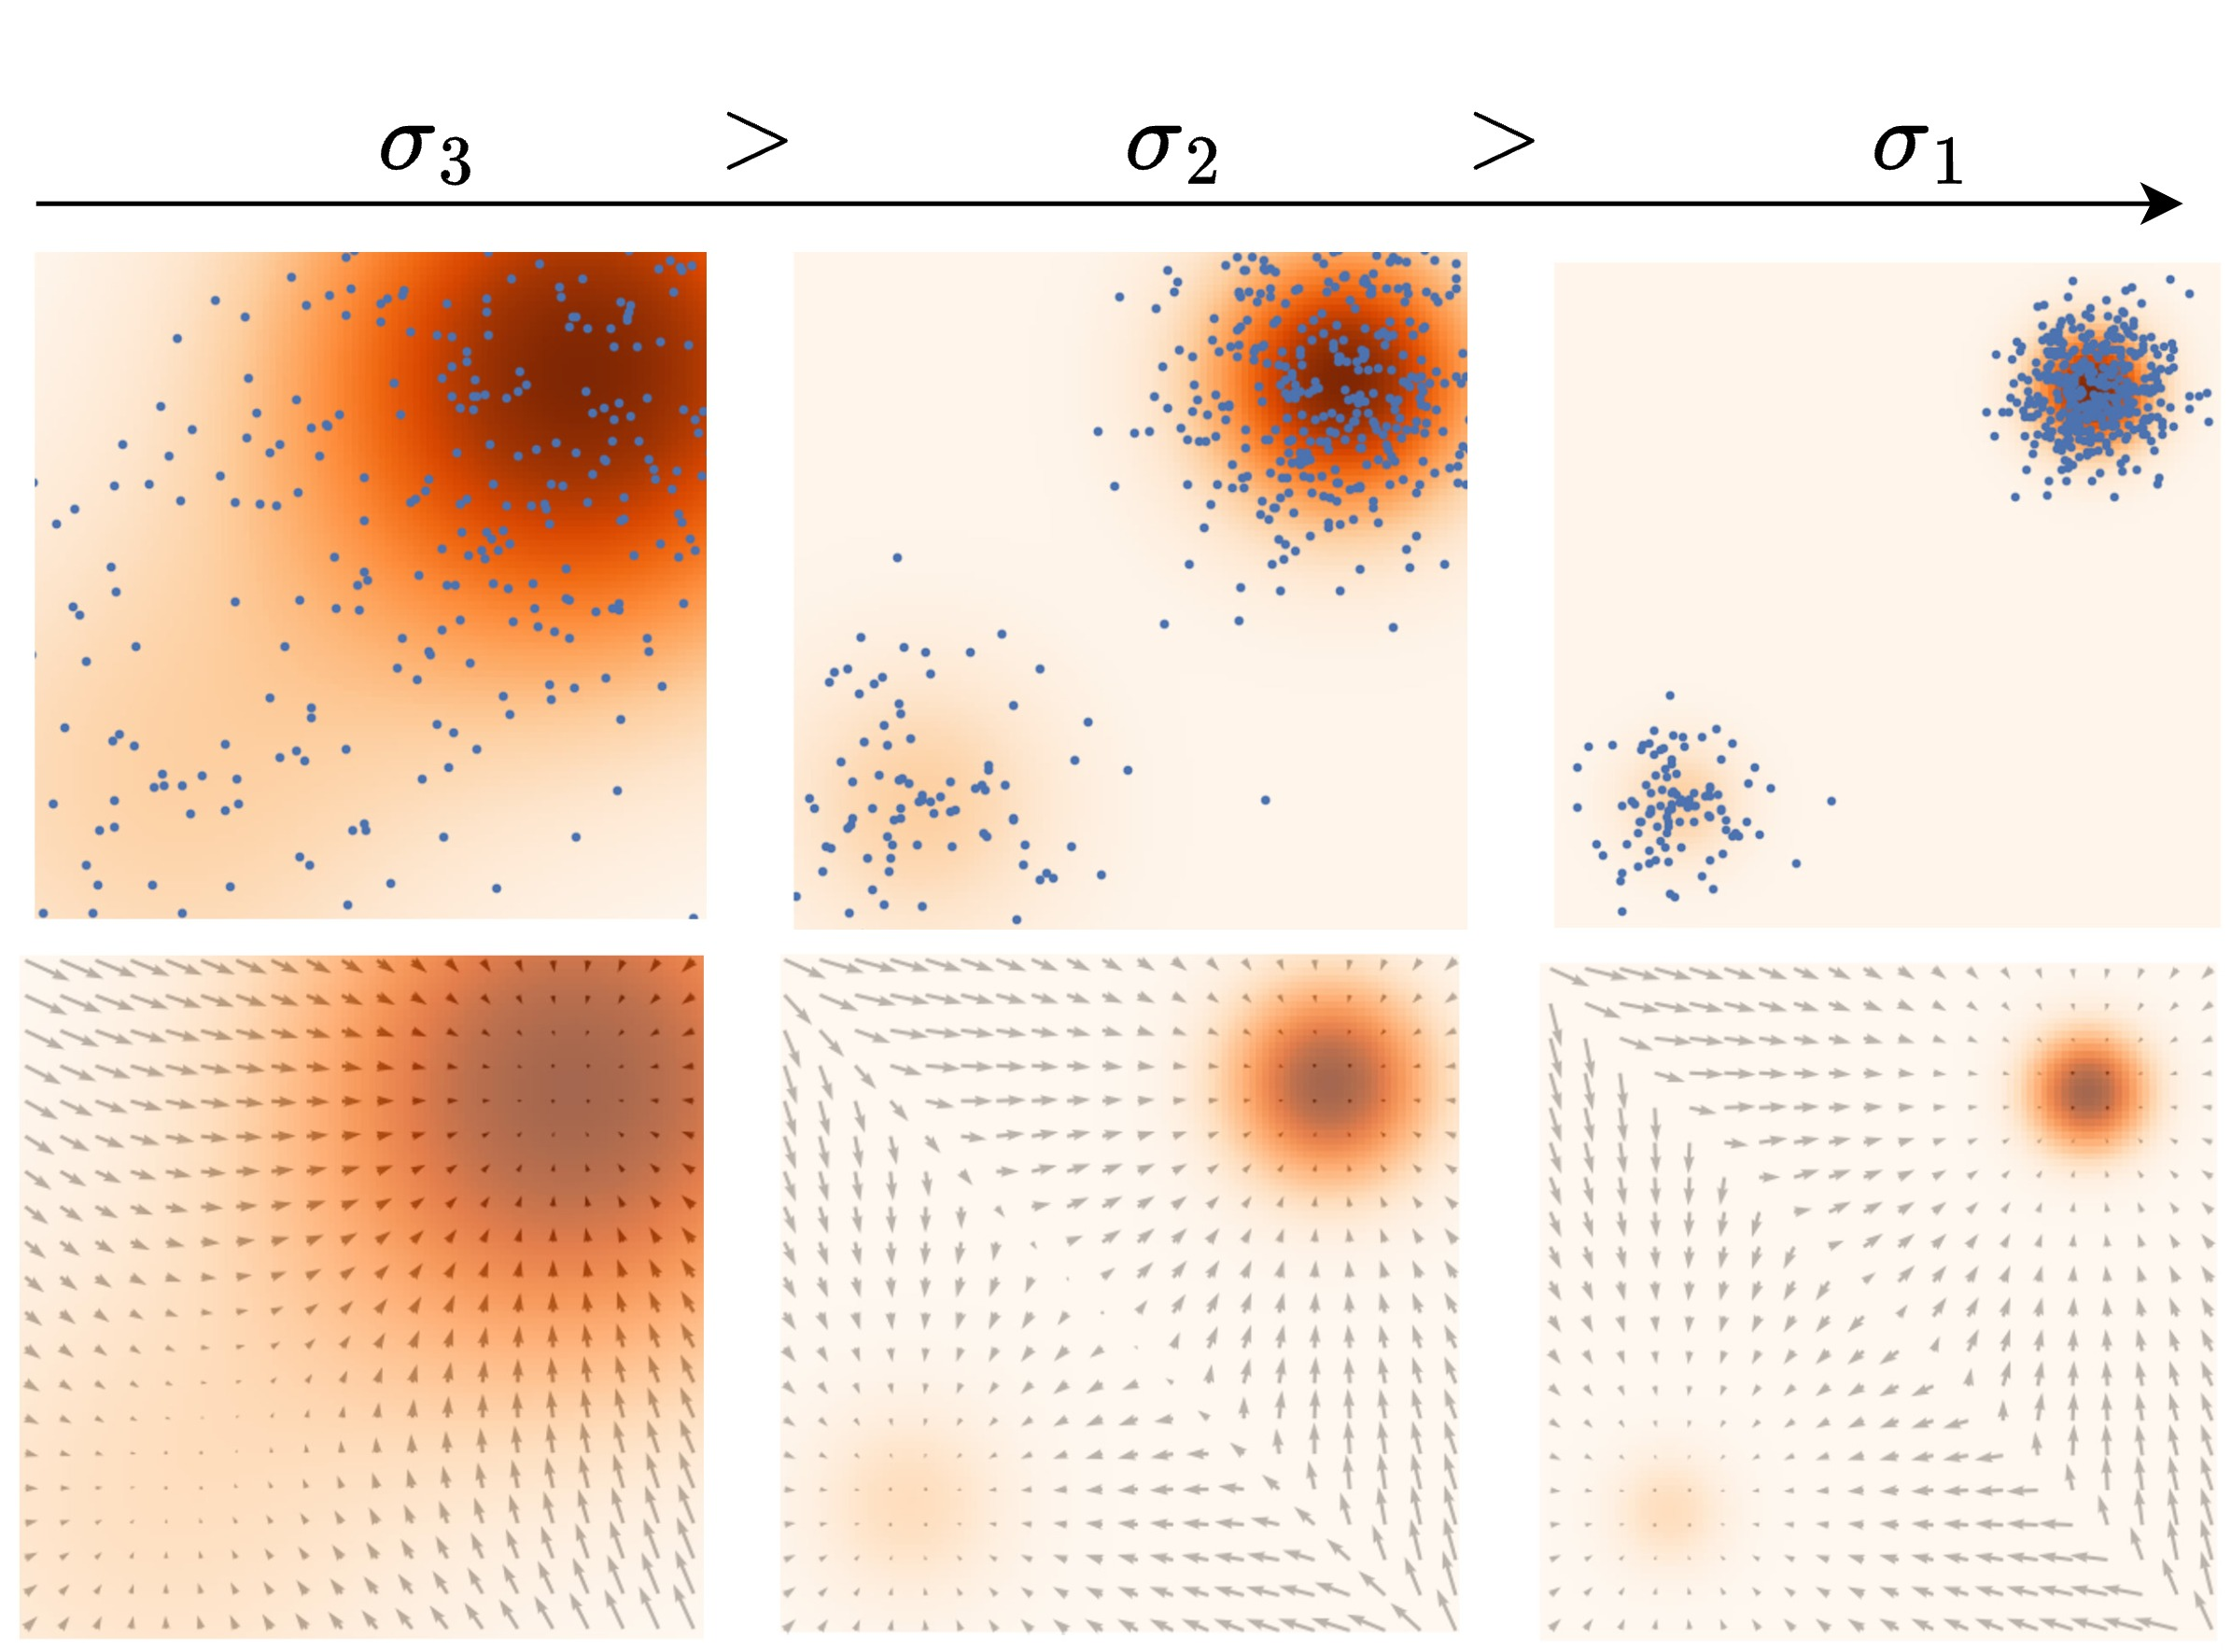
\includegraphics[width=0.9\linewidth]{NoiseScale}
	\end{figure}
\end{frame}

%	Ta gọi $\epsilon = \mathcal{N}(0, I)$
%\begin{columns}
%\begin{column}{0.8\textwidth}
%\begin{figure}
%	\centering
%	\includegraphics[width=\textwidth]{OverviewDiffusion}
%\end{figure}
%\end{column}
%
%\begin{column}{0.2\textwidth}
%
%\end{column}
%\end{columns}
%\\
%q(\mathbf{x}_t \vert \mathbf{x}_{t-1}) &= \mathcal{N}(\mathbf{x}_t; \sqrt{\alpha_t} \mathbf{x}_{t-1}, (1 - \alpha_t)\mathbf{I}) \\ 
%\rightarrow q(\mathbf{x}_t \vert \mathbf{x}_0) &= \mathcal{N}(\mathbf{x}_t; \sqrt{\bar{\alpha}_t} \mathbf{x}_0, (1 - \bar{\alpha}_t)\mathbf{I})


